As described in the last Section, the Bitcoin market price prediction problem in the present work is treated as a binary classification problem. To the best knowledge of the author of the present work, there is no standard dataset that could be applied directly for this purpose. Hence, this Section is concerned with the development of a dataset that can be used for the binary classification of the Bitcoin market price. The basis are day-by-day time series data of the Bitcoin market price as well as related measures that are prepared in the first Subsection. In doing so, features that seem to be usefule for the Bitcoin market price prediction are identified. Then, in the second Subsection, the time series data is transformed into a dataset suitable for binary classification algorithms.

\subsection{Bitcoin Time Series Data}

The Bitcoin time series data is taken from the Blockchain.com API \cite{Data}. In the present work, the time period from \date{01 September 2011} to \date{15 June 2021} is considered. Hence, the time series dataset contains the Bitcoin market price as well as related measures visualized in Fig.~\ref{fig:blockchain.api} for a total of $3576$ days. The Bitcoin market price is reported in $10^4$ USD. It is the average of the Bitcoin trading price of several cryptocurrency exchanges. The market cap is stated in $10^{11}$ USD and describes the value of all Bitcoins that have ever been mined in USD, similar to the market cap of companies at the stock market. The number of transactions is measured in units of $10^5$. The transaction volume - reported in $10^6$ Bitcoin (BTC) - is the total number of Bitcoins transferred per day. The average blocksize in megabyte (MB) as well as the relative difficulty to mine blocks measure the complexity of mining new blocks. The hash rate expressed in $\mathrm{EH} / \mathrm{s}$ is a measure of the computing power that all miners combined are applying. The miner's revenue in $10^7$ USD is the reward that miner's obtain for computing a new block. It is the sum of the newly created Bitcoins and the transaction fees of the transactions in the new block.

\begin{figure}[h!]
  \centering
  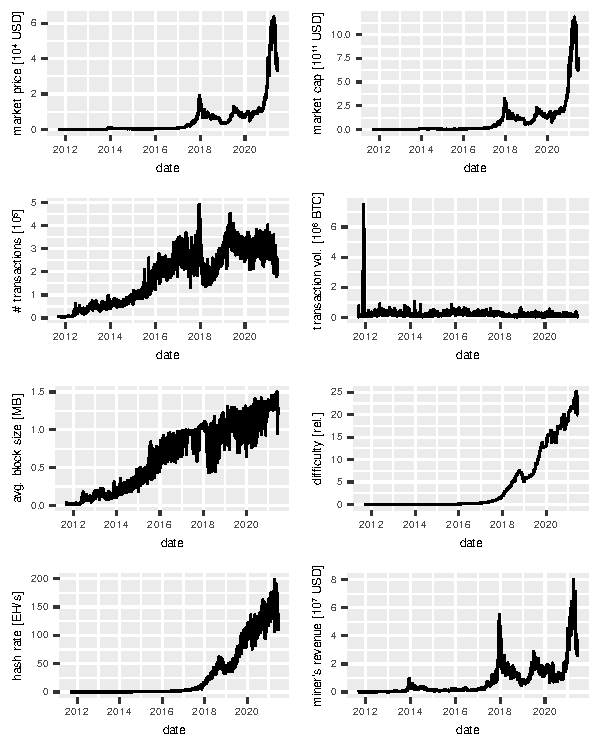
\includegraphics[width=0.9\textwidth]{data.pdf}
  \caption{Bitcoin time series data taken from the Blockchain.com API \cite{Data}. The time series dataset contains information on the Bitcoin market price and the other displayed measures for the time period from \date{01 September 2011} to \date{15 June 2021}. This is a total of $3576$ days. The different measures are explained in the main text.}
  \label{fig:blockchain.api}
\end{figure}

Fig.~\ref{fig:correlation_matrix} shows the correlation matrix of the above described time series dataset. The diagonal - that is the correlation of each time series to itself - is not displayed. The stated values are Pearson's correlation coefficient. The market cap, the difficult, and the miner's revenue reveal a rather high correlation with the market price. These measures are thus not further considered because they do not appear to contain additional information that might be helpful in the prediction of the future Bitcoin market price. In contrast, the transaction volume seems to be uncorrelated to the market price and the other measures. It is also dropped. \\

In Fig.~\ref{fig:all_vs_all}, an overview of the remaining measures that seem to be useful for the prediction of the future Bitcoin market price are displayed.

\begin{figure}[h!]
  \centering
  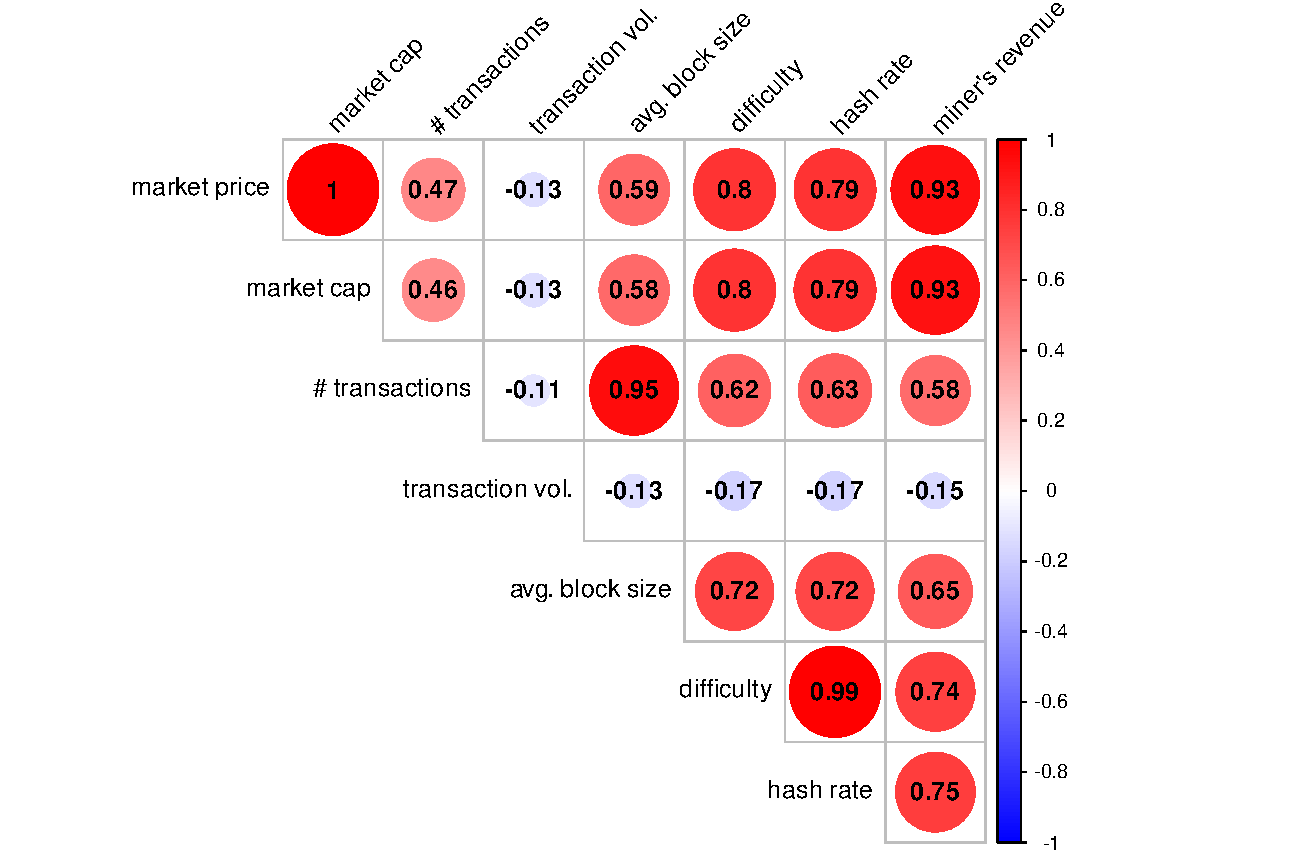
\includegraphics[width=\textwidth]{cor_mat.pdf}
  \caption{Correlation matrix of the time series from Fig.~\ref{fig:blockchain.api}. The displayed values are Pearson's correlation coefficient. Due to their high correlation to the Bitcoin market price, the time series of the market cap, the difficulty, and the miner's revenue are not further considered. In addition, the transaction volume is dropped because it has only a weak correlation to the Bitcoin market price. An overview of the remaining measures can be found in Fig.~\ref{fig:all_vs_all}.}
  \label{fig:correlation_matrix}
\end{figure}

\begin{figure}[h!]
	\centering
	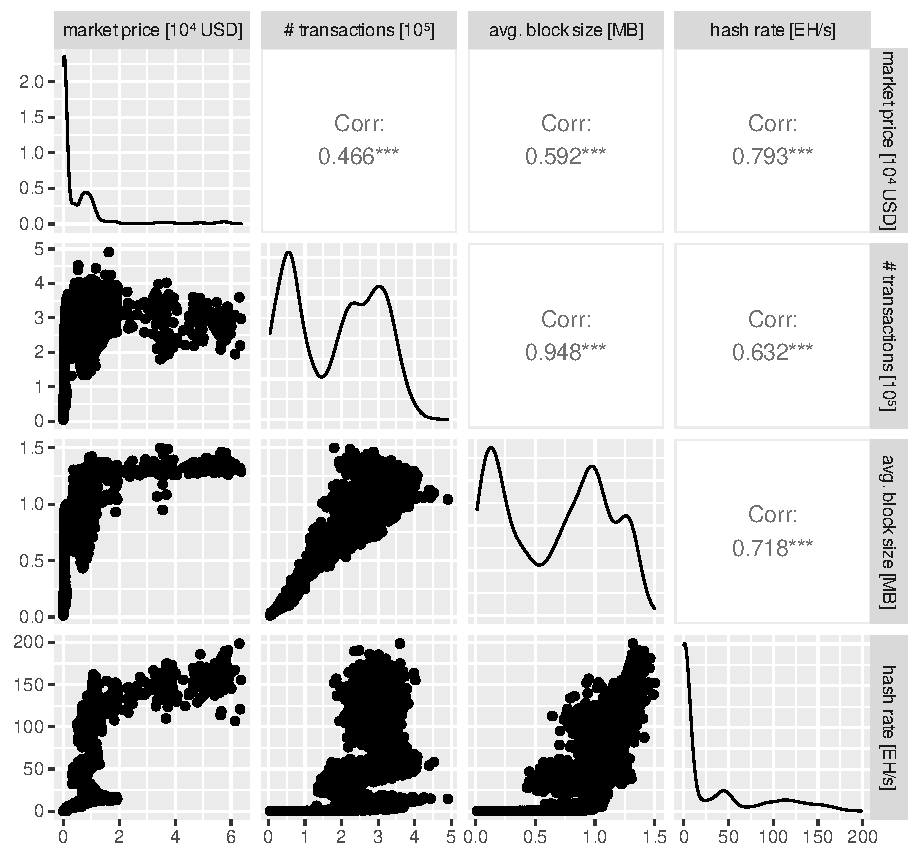
\includegraphics[width=\textwidth]{all_vs_all.pdf}
    \caption{Plot matrix of further considered measures that appear to be useful for the prediction of the future Bitcoin market price. The line plots on the diagonal are the densities of the respective measures. In addition, Pearson's correlation coefficient - the same from Fig.~\ref{fig:correlation_matrix} - is shown. It is observed that the number of transactions, the average block size, and the hash rate reveals a significant correlation to the market price.}
    \label{fig:all_vs_all}
\end{figure}

Finally, Fig.~\ref{fig:autocorrelation} shows the autocorrelation of the Bitcoin market price. It is a measure for how much the Bitcoin market price is related to itself for a given lag. 

\begin{figure}[h!]
	\centering
	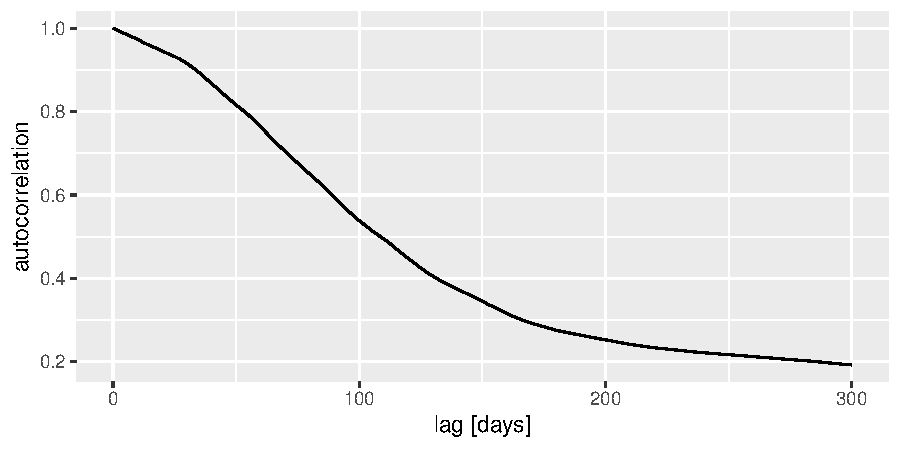
\includegraphics[width=\textwidth]{autocorrelation.pdf}
    \caption{Autocorrelation of the Bitcoin market price. The Bitcoin market price has an autocorrelation larger than $0.5$ for a lag of $100$ days. It is expected that prediction algorithms make use of this time interval for their predictions.}
    \label{fig:autocorrelation}
\end{figure}

\clearpage

\subsection{Transformation to Binary Classification Dataset}
To transform the time series dataset developed in the last Subsection into a dataset suitable for binary classification, the so-called moving-window approach (also called sliding-window approach) is used. For this purpose, the first $m$ days of the time series dataset for all four measures are taken. The last day of this window is taken apart as the future. The other days are taken as the features. The future day is labeled with a $1$, if the Bitcoin price increases with respect to the last, and with a $0$, if it decreases. In the following, the labels $1$ and \enquote{up}, and $0$ and \enquote{down} are used synonymously. In the present work, $m = 100$ is chosen. All of the four features (that are parts of the overall time series dataset) are standardized using the min-max-transformation
\begin{align*}
	\hat{y} = \frac{y - \min(y)}{\max(y) - \min(y)}.
\end{align*}
The examples in the binary classification dataset have the form displayed in Fig.~\ref{fig:example}. There is the historical data for $m-1$ days on the four selected time series including the Bitcoin market price development. The label is the Bitcoin market price direction on the next day. In total, $3477$ examples are generated by using the moving window technique.

\begin{figure}
	\centering
	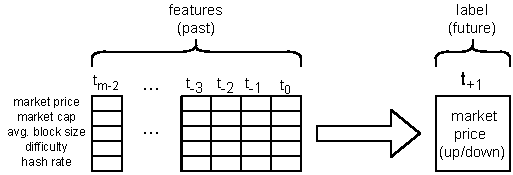
\includegraphics[width=\textwidth]{moving_window.pdf}
    \caption{Example from the binary classification dataset on the Bitcoin market price direction. The features include the past Bitcoin market price and the three selected time series. The label is the Bitcoin market price direction one day into the future.}
    \label{fig:example}
\end{figure}

Finally, the binary classification dataset is split into a training and a test set. Before, all examples in the binary classification dataset are randomly permutated. The split is \SI{80}{\percent} training examples and \SI{20}{\percent} test examples. For more information on the split of the binary classification dataset into a training and a test part, see Subsection~\ref{fig:all_vs_all} of the next Section that contains the theory part of the present work. An overview of the split of the binary classification dataset into training and test examples is given in Fig.~\ref{fig:test}.

\begin{figure}
\centering
\begin{subfigure}{.5\textwidth}
  \centering
  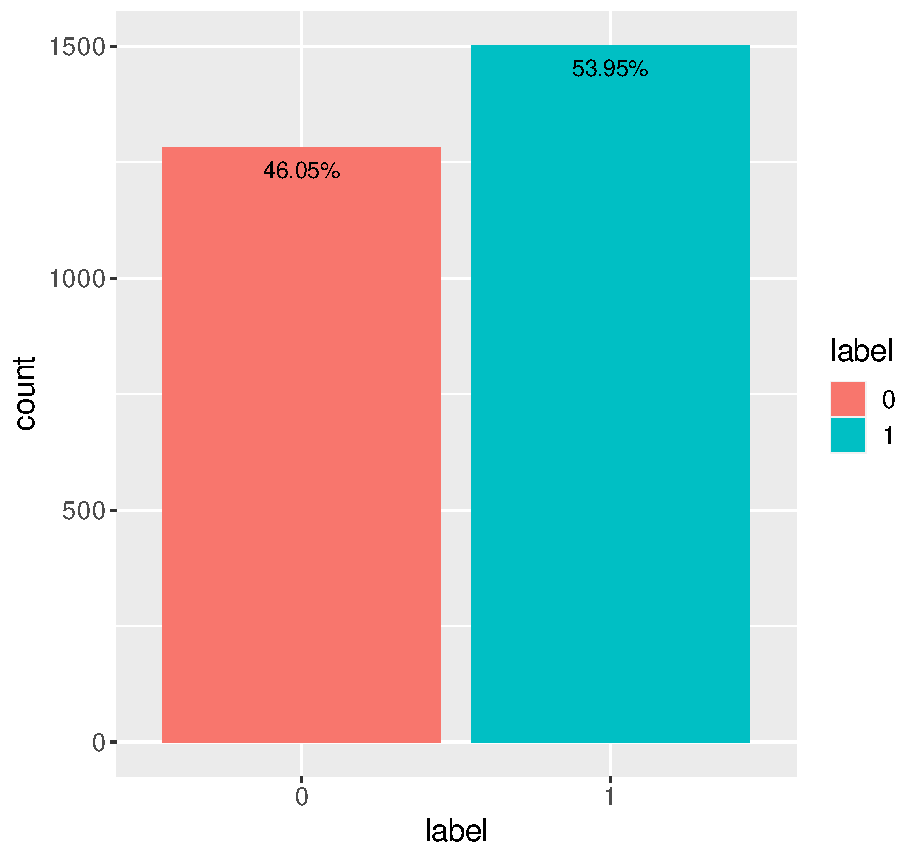
\includegraphics[width=\linewidth]{balance_train.pdf}
  \caption{training examples}
  \label{fig:sub1}
\end{subfigure}%
\begin{subfigure}{.5\textwidth}
  \centering
  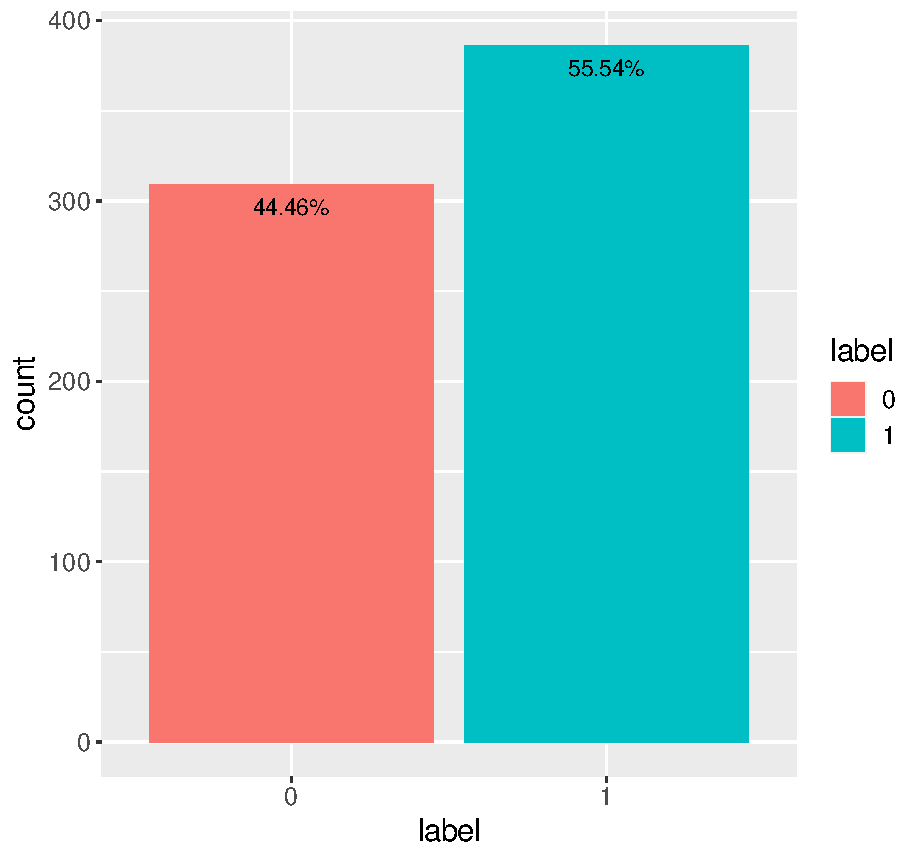
\includegraphics[width=\linewidth]{balance_test.pdf}
  \caption{test examples}
  \label{fig:sub2}
\end{subfigure}
\caption{Split of the binary classification dataset into a training and a test part. Both sets are balanced because the contain both labels roughly the same times.}
\label{fig:test}
\end{figure}

\clearpage